\printconcepts

\exercise{A fundamental calculus technique is to use \underline{\hskip .5in} to refine approximations to get an exact answer.}{limits}

\exercise{What is the upper bound in the summation $\ds \sum_{i=7}^{14} (48i-201)$?}{14}

\exercise{This section approximates definite integrals using what geometric shape?}{Rectangles.}

\exercise{T/F: A sum using the Right Hand Rule is an example of a Riemann Sum.}{T}

\printproblems

\exercisesetinstructions{, write out each term of the summation and compute the sum.}

\exercise{$\ds \sum_{i=2}^{4} i^2$}{$2^2+3^2+4^2 = 29$}

\exercise{$\ds \sum_{i=-1}^{3} (4i-2)$}{$-6-2+2+6+10=10$}

\exercise{$\ds \sum_{i=-2}^{2} \sin (\pi i/2)$}{$0-1+0+1+0 = 0$}

\exercise{$\ds\sum_{i=1}^{10}5$}{$5+5+5+5+5+5+5+5+5+5=50$}

\exercise{$\ds \sum_{i=1}^{5} \frac1i$}{$1+1/2+1/3+1/4+1/5 = 137/60$}

\exercise{$\ds \sum_{i=1}^{6} (-1)^ii$}{$-1+2-3+4-5+6=3$}

\exercise{$\ds \sum_{i=1}^{4} \left(\frac{1}{i} - \frac{1}{i+1}\right)$}{$1/2+1/6+1/12+1/20=4/5$}

\exercise{$\ds \sum_{i=0}^{5} (-1)^i\cos (\pi i)$}{$1+1+1+1+1+1=6$}

\exercisesetend


\input{exercises/05-03-exset-02}

\begin{exerciseset}{In Exercises}{, evaluate the summation using \autoref{thm:summation}.}

\exercise{$\ds \sum_{i=1}^{10} 5$}{50}

\exercise{$\ds \sum_{i=1}^{25} i$}{325}

\exercise{$\ds \sum_{i=1}^{10} (3i^2-2i)$}{1045}

\exercise{$\ds \sum_{i=1}^{15} (2i^3-10)$}{28,650}

\exercise{$\ds \sum_{i=1}^{10} (-4i^3+10i^2-7i+11)$}{$-8525$}

\exercise{$\ds \sum_{i=1}^{10} (i^3-3i^2+2i+7)$}{$2050$}

\exercise{$1+2+3+ \dotsb + 99+100$}{$5050$}

\exercise{$1+4+9+ \dotsb +361+400$}{$2870$}

\end{exerciseset}


\input{exercises/05-03-exset-04}

\exercisesetinstructions{, express the limit as a definite integral.}

\exercise{$\ds \lim_{n\to\infty} \frac{\pi}{n} \sum_{i=1}^n \frac{\sin \frac{\pi i}{n}}{1+\frac{\pi i}{n}}$}{$\ds \int_0^{\pi} \frac{\sin x}{1+x}\dd x$}

\exercise{$\ds \lim_{n\to\infty} \sum_{i=1}^n \frac{3}{n} \biggl(2+\frac{3i}{n}\biggr)\sqrt{1+\biggl(2+\frac{3i}{n}\biggr)^3}$}{$\ds \int_2^5 x\sqrt{1+x^3}\dd x$}

\exercise{$\ds \lim_{n\to\infty} \frac{5}{n} \sum_{i=1}^n \biggl(5\biggl(2+\frac{5i}{n}\biggr)^3-4\biggl(2+\frac{5i}{n}\biggr)+7\biggr)$}{$\ds \int_2^7 5x^3-4x+7\dd x$}

\exercise{$\ds  \lim_{n\to\infty} \frac{2}{n} \sum_{i=1}^n \frac{1+\frac{2i}{n}}{\biggl(1+\frac{2i}{n}\biggr)^2+4}$}{$\ds \int_1^3 \frac{x}{x^2+4}\dd x$}

\exercisesetend

\exercisesetinstructions{, express the definite integral as a limit of a sum.}

\exercise{$\ds \int_2^5 4-2x\dd x$}{$\ds \lim_{n\to\infty}\left[\frac{3}{n} \sum_{i=1}^n 4-2\biggl(2+\frac{3i}{n}\biggr)\right]$}

\exercise{$\ds \int_{-2}^0 x^2+3x\dd x$}{$\ds \lim_{n\to\infty} \frac{2}{n} \sum_{i=1}^n \biggl[\biggl(-2+\frac{2i}{n}\biggr)^2+3\biggl(-2+\frac{2i}{n}\biggr)\biggr]$}

\exercise{$\ds \int_{-\pi/2}^{\pi/2} \frac{\sin^3 x}{2+\cos x}\dd x$}{$\ds \lim_{n\to\infty} \frac{\pi}{n} \sum_{i=1}^n \frac{\sin^3(-\pi/2+\pi i/n)}{2+\cos (-\pi/2+\pi i/n)}$}

\exercise{$\ds\int_0^2 e^x\dd x$}{$\ds\lim_{n\to\infty}\frac2n\sum_{i=1}^n e^{2i/n}$}

\exercisesetend

\exercisesetinstructions{, a definite integral $\ds \int_a^b f(x)\dd x$ is given. 
\begin{enumerate}
\item Graph $f(x)$ on $[a,b]$.
\item Add to the sketch rectangles using the provided rule.
\item Approximate $\ds \int_a^b f(x)\dd x$ by summing the areas of the rectangles.
\end{enumerate}}

\exercise{$\ds \int_{-3}^3 x^2\dd x$, with 6 rectangles using the Left Hand Rule.}{$19$}

\exercise{$\ds \int_{0}^2 (5-x^2)\dd x$, with 4 rectangles using the Midpoint Rule.}{$59/8$}

\exercise{$\ds \int_{0}^\pi \sin x\dd x$, with 6 rectangles using the Right Hand Rule.}{$\pi/3+\pi/(2\sqrt{3}) \approx 1.954$}

\exercise{$\ds \int_1^3 \sqrt{10-x^2}\dd x$ with 4 rectangles using the Right Hand Rule.}{%2.78388+2.44949+1.93649+1=
$8.16986$}

% cut for parity
%\exercise{$\ds \int_{0}^3 2^x\dd x$, with 5 rectangles using the Left Hand Rule.}{$8.144$}

\exercise{$\ds \int_{1}^2 \ln x\dd x$, with 3 rectangles using the Midpoint Rule.}{$0.388584$}

\exercise{$\ds \int_{1}^9 \frac1x\dd x$, with 4 rectangles using the Right Hand Rule.}{$496/315\approx 1.5746$}

\exercisesetend


\exercisesetinstructions{, a definite integral $\ds \int_a^b f(x)\dd x$ is given. As demonstrated in Examples \ref{ex_rie9} and \ref{ex_rie10}, do the following.
\begin{enumerate}
\item Find a formula to approximate $\ds \int_a^bf(x)\dd x$ using $n$ subintervals and the provided rule.
\item Evaluate the formula using $n=10$, $100$ and $1,000$.
\item Find the limit of the formula, as $n\to \infty$, to find the exact value of $\ds \int_a^bf(x)\dd x$.
\end{enumerate}}

\exercise{$\ds \int_{0}^1 x^3\dd x$, using the Right Hand Rule.}{\mbox{}\\[-2\baselineskip]\parbox[t]{\linewidth}{\begin{enumext}
\item Exact expressions will vary; $\frac{(1+n)^2}{4n^2}$.
\item $121/400$, $10201/40000$, $1002001/4000000$
\item $1/4$
\end{enumext}}}

\exercise{$\ds \int_{-1}^1 3x^2\dd x$, using the Left Hand Rule.}{\mbox{}\\[-2\baselineskip]\parbox[t]{\linewidth}{\begin{enumext}
\item Exact expressions will vary; $2+4/n^2$.
\item $51/25$, $5001/2500$, $500001/250000$
\item $2$
\end{enumext}}}

\exercise{$\ds \int_{-1}^3 (3x-1)\dd x$, using the Midpoint Rule.}{\mbox{}\\[-2\baselineskip]\parbox[t]{\linewidth}{\begin{enumext}
\item 8.
\item 8, 8, 8
\item $8$
\end{enumext}}}

\exercise{$\ds \int_{1}^4 (2x^2-3)\dd x$, using the Left Hand Rule.}{\mbox{}\\[-2\baselineskip]\parbox[t]{\linewidth}{\begin{enumext}
\item Exact expressions will vary; $20/3-96/(3n)+64/(3n^2)$.
\item $92/25$, $3968/625$, $103667/15625$
\item $20/3$
\end{enumext}}}

\exercise{$\ds \int_{-10}^{10} (5-x)\dd x$, using the Right Hand Rule.}{\mbox{}\\[-2\baselineskip]\parbox[t]{\linewidth}{\begin{enumext}
\item Exact expressions will vary; $100-200/n$.
\item $80$, $98$, $499/5$
\item $100$
\end{enumext}}}

\exercise{$\ds \int_{0}^{1} (x^3-x^2)\dd x$, using the Right Hand Rule.}{\mbox{}\\[-2\baselineskip]\parbox[t]{\linewidth}{\begin{enumext}
\item Exact expressions will vary; $-(1-1/n^2)/12$.
\item $-33/400$, $-3333/40000$, $-333333/4000000$
\item $-1/12$
\end{enumext}}}

\exercisesetend


\exercise{Use six rectangles to approximate the area under the given graph of $f$ from $x=0$ to $x=12$, using:
\begin{enumerate}
\item The Left Hand Rule,
\item The Right Hand Rule,
\item The Midpoint Rule.
\end{enumerate}
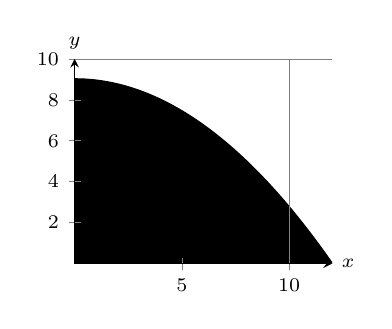
\begin{tikzpicture}
\begin{axis} [width=.4\textwidth,
tick label style={font=\scriptsize},axis y line=middle,axis x line=middle,
name=myplot,axis on top,%all axes={grid},
                        ymin=0,ymax=10,
                        xmin=0,xmax=12,smooth]
   \addplot [draw={\coloronefill},fill=\coloronefill,area style,domain=0:12] {9-(x/4)^2} \closedcycle;
   \addplot [smooth,thick,draw={\colorone},domain=0:12] {9-(x/4)^2};
   \draw [help lines,step=10] (axis cs:0,0) grid (axis cs:12,10);
   % steps=10 was guess and check
\end{axis}
\node [right] at (myplot.right of origin) {\scriptsize $x$};
\node [above] at (myplot.above origin) {\scriptsize $y$};
\end{tikzpicture}}{\mbox{}\\[-2\baselineskip]\parbox[t]{\linewidth}{\begin{enumerate}
\item	Exact expressions will vary; $80.5$.
\item	$72.25$
\item	$62.5$
\end{enumerate}}}

\exercise{A car accelerates from 0 to 40 mph in 30 seconds. The speedometer reading at each 5 second interval during this time is given in the table below. Estimate how far the car travels during this 30 second period using the velocities at:
\begin{enumerate}
\item The beginning of each time interval.
\item The end of each time interval.
\end{enumerate}

\begin{center}
\begin{tabular} {|c|c|c|c|c|c|c|c|}
\hline
$t$ (sec)&0&5&10&15&20&25&30\\ \hline
$v$ (mph)&0&6&14&23&30&36&40\\ \hline
\end{tabular}
\end{center}}{\mbox{}\\[-2\baselineskip]\parbox[t]{\linewidth}{\begin{enumerate}
\item	$(5\text{ s})((0+6+14+23+30+36)\text{ mph})=545\frac{\text{mi s}}{\text{hr}}\times\frac{1\text{ hr}}{3600\text{ s}}\times{5280\text{ ft}}{1\text{ mi}}=799\text{ ft}$
\item	$(5\text{ s})((6+14+23+30+36+40)\text{ mph})=585\frac{\text{mi s}}{\text{hr}}\times\frac{1\text{ hr}}{3600\text{ s}}\times{5280\text{ ft}}{1\text{ mi}}=858\text{ ft}$
\end{enumerate}}}

\exercise{Use Theorems \ref{thm:summation} and \ref{thm:riemannSum} to justify the remaining property in \autoref{thm:defintprop}: \[\int_a^b k\cdot f(x)\dd x =k\int_a^b f(x)\dd x\]}{\mbox{}\\[-2\baselineskip]\parbox[t]{\linewidth}{\begin{align*}
\int_a^b k\cdot f(x)\dd x
&=\lim_{n\to\infty}\sum_{i=1}^n k\cdot f(c_i)\Delta x
\quad\text{T\ref{thm:riemannSum}.2} \\
&=\lim_{n\to\infty}k\cdot\sum_{i=1}^n k\cdot f(c_i)\Delta x
\quad\text{T\ref{thm:summation}.3} \\
&=k\cdot\lim_{n\to\infty}\sum_{i=1}^n k\cdot f(c_i)\Delta x
\quad\text{T\ref{thm:limit_algebra}.4} \\
&=k\int_a^b f(x)\dd x\quad\text{T\ref{thm:riemannSum}.2}
\end{align*}}}

\exercise{Use Theorems \ref{thm:summation} and \ref{thm:riemannSum} to justify the remaining property in \autoref{thm:further_def_int_props}: If $f(x)\leq M$ for all $x$ in $[a,b]$, then
\[\int_a^b f(x)\dd x\leq M(b-a).\]}{Let $f$ and $M$ be as given.
\begin{align*}
\int_a^b f(x)\dd x
&=\lim_{n\to\infty}\sum_{i=1}^n f(c_i)\Delta x
\quad\text{T\ref{thm:riemannSum}.2} \\
&\le\lim_{n\to\infty}\sum_{i=1}^n M\Delta x \\
&=\int_a^b M\dd x\quad\text{T\ref{thm:riemannSum}.2} \\
&=M(b-a)
\end{align*}}

\printreview

\begin{exerciseset}{In Exercises}{, find an antiderivative of the given function.}

\exercise{$f(x) = 5\sec^2 x$}{$F(x) = 5\tan x+ 4$}

\exercise{$\ds f(x) = \frac7x$}{$F(x) = 7\ln\abs x + 14$}

\exercise{$\ds g(t) = 4t^5-5t^3+8$}{$G(t) = 4/6t^6-5/4t^4+8t+9$}

\exercise{$\ds g(t) = 5\cdot e^t$}{$G(t) = 5\cdot e^t + 900$}

\exercise{$\ds g(t) = \cos t + \sin t$}{$G(t) = \sin t-\cos t -78$}

\exercise{$\ds f(x) = \frac{1}{\sqrt{x}}$}{$F(x) = 2\sqrt{x} -\pi$}

\end{exerciseset}

